% Relatorio do trabalho de Circuitos Eletricos II 2018.1

\documentclass[11pt,titlepage]{article}

\usepackage[utf8]{inputenc}
\usepackage[T1]{fontenc}
\usepackage[portuguese]{babel}
\usepackage{fancyvrb}
\usepackage{enumitem}

\usepackage{titlepic}
\usepackage{graphicx}
\usepackage[justification=centering, labelfont=bf]{caption}
\usepackage[margin=1.5in]{geometry}

\usepackage[americanvoltage,betterproportions]{circuitikz}

% Capa do relatorio
\title{\textbf{Projeto de um Programa de Análise Nodal Modificada Compacta no Tempo}\\
\medskip
\large Trabalho de Circuitos Elétricos II - 2018.1}

\author{
  Matheus Fernandes Moreno\\
  \texttt{116038745}
  \and
  Paulo Victor S. Pedroso de Lima\\
  \texttt{115203101}
}

\date{\bigskip
Professor: Antônio Carlos Moreirão de Queiroz\\
\smallskip
Departamento de Engenharia Eletrônica e de Computação\\
\smallskip
Universidade Federal do Rio de Janeiro - Escola Politécnica\\
\bigskip
Junho de 2018}

\titlepic{
\includegraphics[width=90pt]{simbolo_ufrj.png}}
% Fim da capa

\begin{document}

\maketitle

\newpage
\tableofcontents


\newpage
\section{Introdução}

Este relatório é composto de comentários e demonstrações acerca do trabalho do período de 2018.1 da cadeira Circuitos Elétricos II (ministrada pelo professor Antônio Carlos Moreirão de Queiroz, no curso de Engenharia Eletrônica e de Computação) desenvolvido pelos autores.

O projeto consistiu na implementação de um programa capaz de realizar a análise de circuitos lineares e não lineares no domínio no tempo. Para isso, foi utilizado o método de análise nodal modificada compacta (simplificação por modelos com amplificadores operacionais, que não aumentam a ordem do sistema) e o \textquotedbl método $\theta$\textquotedbl{} de integração, juntamente com o método de Newton-Raphson para a resolução de casos não lineares.

O programa foi desenvolvido na linguagem C e, para testar seu funcionamento, foram simulados circuitos com respostas conhecidas e comparados os resultados com o programa MNAE, que implementa a análise no tempo com as mesmas especificações.


\newpage
\section{Resultados}

\subsection{Especificação do Programa}

O programa é capaz de ler um arquivo de \textquotedbl netlist\textquotedbl{} (\texttt{.net}) que descreve os elementos e conexões do circuito a ser analisado. Neste arquivo devem estar todas as especificações necessárias para cada componente da topologia na formatação padronizada.

Os elementos aceitos para análise encontram-se abaixo:

\begin{itemize}[noitemsep]
    \item Resistores (\texttt{R});
    \item Capacitores (\texttt{C});
    \item Indutores (\texttt{L});
    \item Fontes de tensão (\texttt{V}) e corrente (\texttt{I}) independentes, podendo ser contínuas, senoidais ou pulsadas;
    \item As quatro fontes controladas (\texttt{E}, \texttt{F}, \texttt{G}, \texttt{H});
    \item Amplificadores operacionais ideais, com 4 terminais (\texttt{O});
    \item Transformadores ideais (\texttt{K});
    \item Transistores bipolares do tipo NPN e PNP (\texttt{Q});
    \item Diodos (\texttt{D}).
\end{itemize}

Após a leitura do arquivo, o programa calcula o ponto de operação do circuito e realiza a análise com o tempo total, passo fixo e valor de $\theta$ dados (são utilizados valores padrão se estes não forem especificados). Os resultados são salvos em uma tabela (um arquivo do tipo \texttt{.tab}), que pode ser lida por um traçador de curvas. Os gráficos deste relatório foram traçados com o programa MNAE, do professor Antônio Carlos Moreirão.

O projeto foi desenvolvido a partir do código-fonte do programa MNA1AMP, também do prof. Moreirão, que implementa a resolução de circuitos usando a simplificação do sistema por amplificadores operacionais \cite{apostilaCEII}, em C. Neste algoritmo, elementos não aceitos pela análise nodal simples são modelados por fontes de corrente e amp. ops. de tal forma que o tamanho do sistema não aumenta como no caso de uma análise nodal modificada. Ademais, amplificadores operacionais no circuito diminuem o tamanho do sistema.

O \textquotedbl método $\theta$\textquotedbl{} de integração é utilizado para o geração de estampas de capacitores e indutores invariantes no tempo, e consiste na aproximação de integrais por meio da equação

$$y(t_o + \Delta t) = y(t_o) + \int_{t_o}^{t_o + \Delta t}x(t)\mathrm{d}t \approx y(t_o) + \Delta t (\theta x(t_o + \Delta t) + (1 - \theta)x(t_o))$$

que abrange os métodos \textquotedbl backward Euler\textquotedbl{} ($\theta = 1$), \textquotedbl forward Euler\textquotedbl{} ($\theta = 0$) e dos trapézios ($\theta = 0.5$), além dos valores inclusos continuamente entre esses.

O método de Newton-Raphson implementado é iterativo e responsável pela análise dos elementos não lineares aceitos pelo programa (diodos e transistores). São usados modelos linearizados desses elementos, com valores que dependem do resultado da análise anterior, e calculados novos resultados. O controle de convergência para o método foi implementado observando os erros absolutos ou relativos (dependendo da ordem de grandeza do resultado atual) entre iterações do método. Caso não haja convergência após um número razoável de iterações, os valores são randomizados.



\subsection{Exemplos}

A seguir encontram-se alguns exemplos de circuitos que incluem os elementos implementados e apresentam resultados relacionados às especificações do programa. Nas topologias de circuitos osciladores/ressonantes, foram omitidas as fontes responsáveis por \textquotedbl ativar\textquotedbl{} os sistemas; elas, porém, encontram-se em seus respectivos \textquotedbl netlists\textquotedbl{}.

\subsubsection{Memória Falsa e Artefato no Indutor}

Este circuito contém um indutor e um diodo em série, que pode causar a criação de artefatos. Ao aproximarmos a integral do indutor pelo \textquotedbl método $\theta$\textquotedbl{}, geramos uma memória falsa em sua tensão, que deveria depender apenas da variação de corrente, mas passa a depender também da tensão anterior. No instante em que o diodo corta, a corrente no indutor é nula, mas sua tensão não se anula, e é gerada uma tensão com oscilação de alta frequência. Para $\theta \leq 0.5$, o artefato vai ficando mais grave, mantendo-se até que o diodo volte a conduzir.

% Codigo do circuito do artefato
\begin{Verbatim}[frame=single]
Artefato na tensao do indutor
V1 1 0 SIN 0 10 1000 0 0 0 10
L1 1 2 1E-3
D1 2 3 1E-9 4.3429445E-2
R1 3 0 10
.TRAN 2E-3 10E-6 TETA 0.6 1
\end{Verbatim}

% Desenho do circuito artefato
\begin{figure}[!ht]
\centering
\begin{circuitikz} \draw
    (0, 0) node[ground]{}
    (0, 0) to[sV, l=$10\sin({2\pi1000\mathrm{t}}) \mathrm{V}$]
    (0, 2) to[L, l_=$1 \mathrm{mH}$, *-*]
    (2.5, 2) --
    (3.5, 2) to[D]
    (4, 2) --
    (5, 2) to[R, l=$10 \mathrm{\Omega}$, *-] (5,0)
    (5, 0) node[ground]{}
    (0, 2.5) circle (6pt) node[]{1}
    (2.5, 2.5) circle (6pt) node[]{2}
    (5, 2.5) circle (6pt) node[]{3}
    ;
\end{circuitikz}
\caption{Circuito que gera artefato na tensão do indutor.}
\end{figure}

\begin{figure}[!ht]
\centering
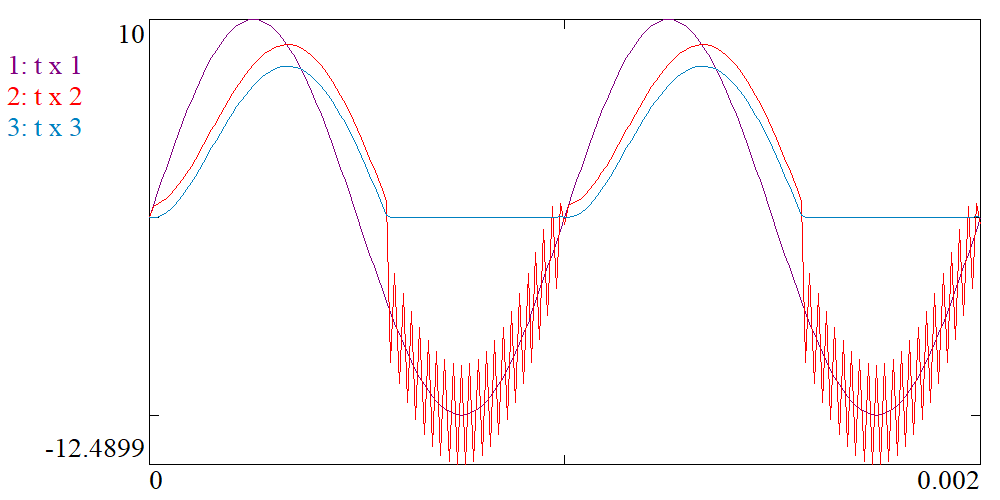
\includegraphics[scale=0.5]{graficos/artefato_trapezio.png}
\caption{Gráfico das tensões nos nós 1, 2 e 3 do circuito gerador de artefato quando usado $\theta = 0.5$ (equivalente ao método dos trapézios).}
\end{figure}

\begin{figure}[!ht]
\centering
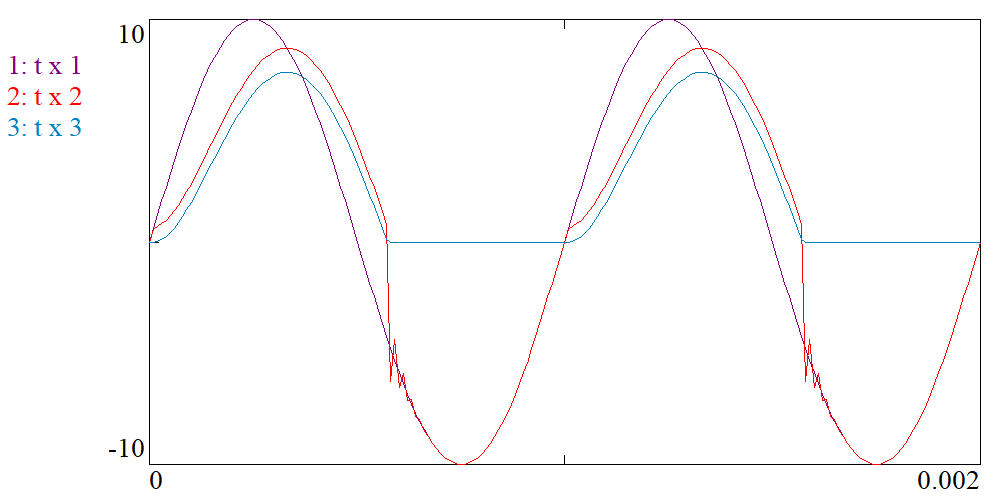
\includegraphics[scale=0.5]{graficos/artefato_06.png}
\caption{Gráfico das tensões nos nós 1, 2 e 3 do mesmo circuito quando usado $\theta = 0.6$. O artefato foi rapidamente amortecido.}
\end{figure}


\subsubsection{Circuito de Chua}

O circuito de Chua é um circuito de natureza caótica. Ele é composto por um indutor, dois capacitores, um resistor linear e um resistor linear por partes (chamado também de \textquotedbl diodo de Chua\textquotedbl{}). O circuito oscila aperiodicamente e, se as tensões sobre cada capacitor forem plotadas uma em função da outra, é possível visualizar um atrator estranho do tipo dupla-espiral \cite{chaotic}.

Como o resistor linear por partes não foi implementado no programa, a curva característica do diodo de Chua foi gerada com um equivalente composto por um conversor de impedância negativa, diodos e resistores.

% Codigo do circuito de Chua
\begin{Verbatim}[frame=single]
Circuito de Chua
R1 1 2 2
R2 3 4 2
R3 5 0 -1.4
R4 6 5 1.9
L1 6 0 1
C1 5 7 0.31
C2 6 8 1
D1 0 2 1e-9 43.429445e-3
D2 5 3 1e-9 43.429445e-3
V1 4 0 DC 2
V2 7 0 PULSE 0 0.1 0 0 0 10000 20000 1
V3 8 0 PULSE 0 0.1 0 0 0 10000 20000 1
V4 1 5 DC 2
.TRAN 1000 100E-3 TETA 0.55 1
\end{Verbatim}

% Desenho do circuito de Chua
\begin{figure}[!ht]
\centering
\begin{circuitikz}[scale=0.8] \draw
    (0, 0) node[ground]{}
    (0, 0) to[L, l=$1 \mathrm{H}$]
    (0, 4) --
    (2, 4) to[C, l_=$1 \mathrm{F}$]
    (2, 0) node[ground]{}
    (2, 4) to[R, l=$1.9 \mathrm{\Omega}$, *-*]
    (4, 4) to[C, l=$0.31 \mathrm{F}$]
    (4, 0) node[ground]{}
    (4, 4) --
    (6.5, 4) to[R, l=$-1.4 \mathrm{\Omega}$]
    (6.5, 0) node[ground]{}
    (6.5, 4) --
    (9, 4) to[D]
    (9, 2) to[R, l=$2\mathrm{\Omega}$]
    (9, 0) to[V, l=$2\mathrm{V}$]
    (9, -2) node[ground]{}
    (12, -2) node[ground]{}
    (12, -2) to[D]
    (12, 0) to[R, l=$2\mathrm{\Omega}$]
    (12, 2) to[V, l=$2\mathrm{V}$]
    (12, 4) -- (9, 4)
    (1.7, 4.5) circle (7pt) node[]{\small{6}}
    (4.3, 4.5) circle (7pt) node[]{\small{5}}
    ;
\end{circuitikz}
\caption{Circuito de Chua com estrutura equivalente para o diodo de Chua.}
\end{figure}

\begin{figure}[!ht]
\centering
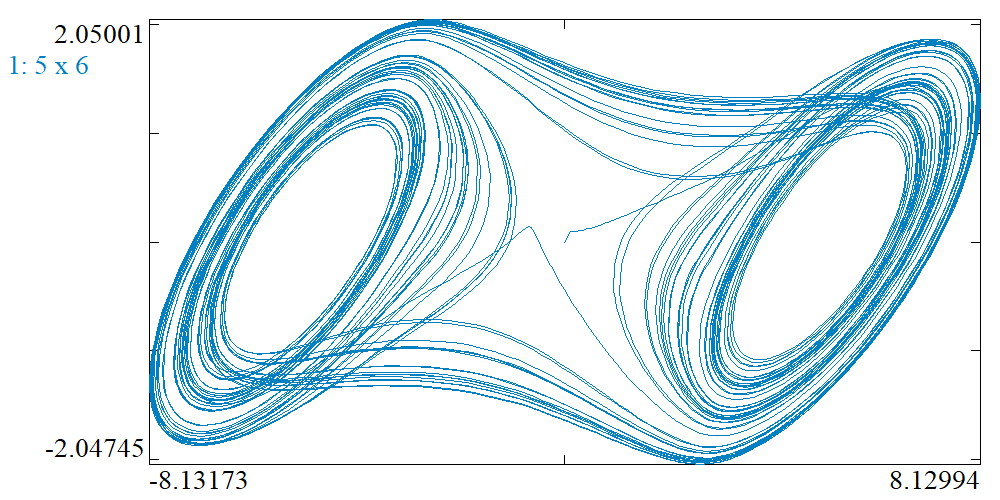
\includegraphics[scale=0.5]{graficos/chua.png}
\caption{Gráfico das tensões nos capacitores do Circuito de Chua. Foram utilizados apenas os últimos 50 segundos de simulação, para facilitar a visualização do gráfico. Observe o atrator de dupla-espiral.}
\end{figure}


\pagebreak
\subsubsection{Tanque LC com Indutor Ativo}

O circuito abaixo é um tanque LC com indutância ativa, composto por um conversor de impedância generalizada (formado pela configuração dos amplificadores operacionais, resistores e capacitor) — que apresentará uma indutância equivalente de $L_{eq} = 100 \mathrm{mH}$ — em paralelo com um capacitor. Observe o efeito do mapeamento do eixo $\jmath\omega$ no plano complexo de acordo com o valor de $\theta$ escolhido: para o método dos trapézios, o sistema mantém sua amplitude de oscilação; para $\theta < 0.5$, o sistema fica estável; e para $\theta > 0.5$, o sistema fica instável.

% Codigo do tanque LC ativo
\begin{Verbatim}[frame=single]
Tanque LC com indutor ativo
I1 1 0 PULSE 0 1E-3 0 0 0 1e-5 2e-5 1
R1 1 2 10000
C1 2 3 1E-9
R2 3 4 10000
R3 4 5 10000
R4 5 0 10000
CX 1 0 68E-9
O1 4 0 1 3
O2 2 0 5 3
.TRAN 6E-3 1E-5 TETA <0.4/0.5/0.6> 1
\end{Verbatim}

% Circuito do tanque LC com indutor ativo
\begin{figure}[!ht]
\centering
\begin{circuitikz}[scale=0.8] \draw
    (1, 0) node[op amp, yscale=-1](O1){}
    (-5, -4) node[op amp, xscale=-1](O2){}
    (O1.-) |- (-2, -2)
    (O1.out) |- (-2, -4)
    (O2.+) |- (-2, -6)
    (O2.-) |- (-2, -2)
    (O2.out) |- (-2, 0)
    (O1.+) |-
    (-2, 2) to[R, l_=$10 \mathrm{k\Omega}$]
    (-2, 0) to[C, l_=$1 \mathrm{nF}$]
    (-2, -2) to[R, l=$10 \mathrm{k\Omega}$]
    (-2, -4) to[R, l=$10 \mathrm{k\Omega}$]
    (-2, -6) to[R, l=$10 \mathrm{k\Omega}$]
    (-2, -8) node[ground]{}
    (-2, 2) --
    (4, 2) to[C, l=$68 \mathrm{nF}$, *-]
    (4, -1) node[ground]{}
    (4, 2) to[short, -o] (5, 2)
    (5.5, 2) node[]{$v_o$}
    ;
\end{circuitikz}
\caption{Tanque LC com indutor ativo gerado por um conversor de impedância generalizado.}
\end{figure}

\begin{figure}[!ht]
\centering
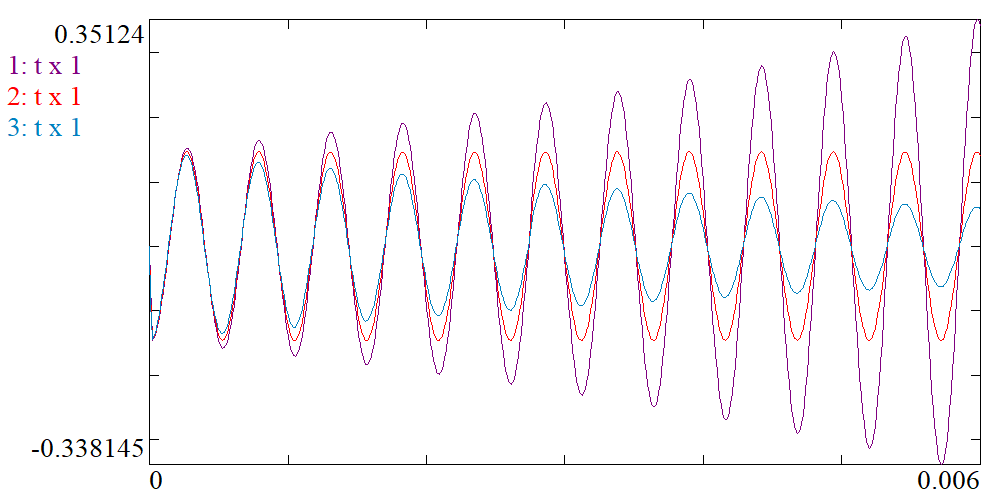
\includegraphics[scale=0.5]{graficos/oscilador_lativo.png}
\caption{Gráfico com os sinais de saída do tanque LC para $\theta = 0.4$, $\theta = 0.5$ e $\theta = 0.6$, respectivamente.}
\end{figure}



\subsubsection{Bobina de Tesla}

A Bobina de Tesla é um circuito ressonante capaz de gerar tensões muito altas. Ela possui uma boa topologia para testar o funcionamento do transformador ideal e dos elementos reativos do programa. Observe no gráfico que há um decaimento da amplitude pois, como mencionado na seção anterior, foi usado $\theta > 0.5$ na simulação.

% Codigo do circuito da bobina de tesla
\begin{Verbatim}[frame=single]
Bobina de Tesla
L1 1 0 1E-5
L2 2 3 1.54797097554421E-4
C1 1 4 1E-8
C2 2 0 6.25E-10
K1 1 0 3 0 7.21311475409836E-1
V1 4 0 PULSE 0 10000 0 0 0 1 2 1
.TRAN 0.5E-4 1E-8 TETA 0.55 1
\end{Verbatim}

% Bobina de tesla
\begin{figure}[!ht]
\centering
\begin{circuitikz} \draw
    (-1, 3) node[ground]{}
    (-1, 3) to[C, l=$10 \mathrm{nF}$]
    (-1, 5) --
    (1, 5) to[L, l=$10 \mathrm{\mu H}$, *-]
    (1, 3) node[ground]{}
    (4, 5) node[transformer core](K1){}
    (K1.A1) -- (1, 5)
    (K1.A2) -| (1, 3)
    (K1.B2) -| (7.5, 3)
    (K1.B1) to[L, l_=$0.155 \mathrm{mH}$]
    (7, 5) --
    (7.5, 5) to[C, l=$0.625 \mathrm{nF}$, *-]
    (7.5, 3) node[ground]{}
    (4.3, 4.52) node[fill=black, circle, scale=0.3]{}
    (3.7, 4.52) node[fill=black, circle, scale=0.3]{}
    (4.42, 5) node[fill=black, circle, scale=0.33]{}
    (1, 5.5) circle (6pt) node[]{1}
    (7.5, 5.5) circle (6pt) node[]{2}
    (4.42, 5.5) circle (6pt) node[]{3}
    ;
\end{circuitikz}
\caption{Circuito da Bobina de Tesla, caso geral.}
\end{figure}

\begin{figure}[!ht]
\centering
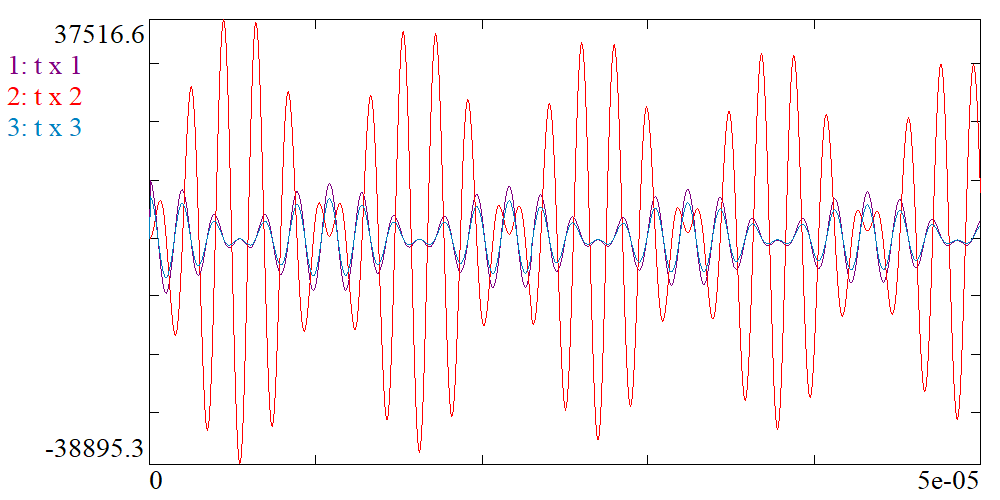
\includegraphics[scale=0.5]{graficos/tesla.png}
\caption{Gráfico das tensões oscilantes na Bobina de Tesla. As amplitudes estão decaindo pois foi usado $\theta$ > 0.5.}
\end{figure}



\subsubsection{Retificador de Onda Completa}

Este circuito trata-se de um retificador de onda completa, composto de diodos, resistores e amplificadores operacionais. Sua grande utilidade deve-se ao fato de possibilitar a retificação de sinais de baixas amplitudes, onde a tensão é menor que a tensão de joelho dos diodos. Nestas condições, outros retificadores que não são compostos por amplificadores seriam incapazes de funcionar.

% Codigo do retificador
\begin{Verbatim}[frame=single]
Retificador de onda completa
V1 1 0 SIN 0 100e-3 5 0 0.2 0 5
R1 1 2 2000
R2 1 5 2000
R3 2 4 2000
R4 4 5 1000
R5 5 6 2000
RL 6 0 1000
D1 4 3 1E-9 4.3429445E-2
D2 3 2 1E-9 4.3429445E-2
O1 3 0 0 2
O2 6 0 0 5
.TRAN 1 1e-4 TETA 0.5 1
\end{Verbatim}

% Retificador de onda completa
\begin{figure}[!ht]
\centering
    \begin{circuitikz}[scale=0.9] \draw
    (-0.5, 0) node[ground]{}
    (3, 2.5) node[op amp, yscale=-1](O1){}
    (10.5, 3.05) node[op amp, yscale=-1](O2){}
    (O1.+) -|
    (1.5, 2.95) node[ground]{}
    (-0.5, 0) to[sV, l=V1]
    (-0.5, 1.95) to[R, l_=$2 \mathrm{k\Omega}$] (O1.-)
    (O1.out) --
    (4.5, 2.5) --
    (4.5, 1) to[D]
    (1.8, 1) -- (1.8, 1.95)
    (6, 2.5) to[D] (4.5, 2.5)
    (6, 2.5) to[R, l_=$1 \mathrm{k\Omega}$]
    (8, 2.5) --
    (8, 4) to[R, l_=$2 \mathrm{k\Omega}$]
    (-0.5, 4) -- (-0.5, 1.95)
    (6, 2.5) --
    (6, 0) to[R, l=$2 \mathrm{k\Omega}$]
    (1.8, 0) -- (1.8, 1)
    (O2.-) -- (8, 2.5)
    (O2.+) -|
    (9, 3.5) node[ground]{}
    (8.5, 2.5) --
    (8.5, 1.5) to[R, l_=$2 \mathrm{k\Omega}$]
    (11, 1.5) -| (O2.out)
    (11.82, 1.5) to[R, l_=$1 \mathrm{k\Omega}$]
    (11.82, -0.5) node[ground]{}
    (11.82, 1.5) to[short, -o] (12.69, 1.5)
    (13.1, 1.5) node[]{$v_o$}
    ;
    \end{circuitikz}
\caption{Retificador de onda completa para sinais de baixa amplitude.}
\end{figure}

\begin{figure}[!ht]
\centering
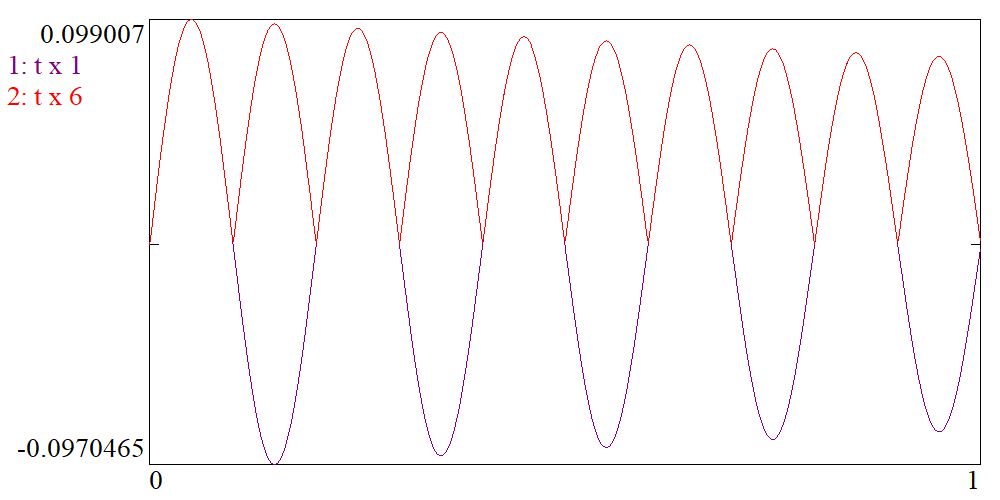
\includegraphics[scale=0.5]{graficos/retificador.png}
\caption{Entrada e saída do retificador de onda completa.}
\end{figure}



\subsubsection{Traçador de Curvas do Transistor}

Um método para verificar o modelamento dos transistores é simulando um circuito traçador de curvas como o apresentado a seguir. Uma fonte de tensão pulsada é especificada de tal forma que funcione como uma onda triangular, variando a tensão do coletor ao emissor do transistor, ao passo que fontes de corrente pulsadas aumentam periodicamente o valor de $i_b$. Colocando uma fonte de tensão controlada pela corrente $i_c$ de ganho unitário, podemos plotar as curvas características dos transistores NPN e PNP, $v_{CE} \times i_c$.

% Codigo do tracador de curvas
\begin{Verbatim}[frame=single]
Tracador de curvas do transistor
Q1 1 6 0 NPN 0.99 0.5 3.77513E-14 0.025 3.77513E-14 0.025 1E9
Q2 3 8 0 PNP 0.99 0.5 3.77513E-14 0.025 3.77513E-14 0.025 1E9
H1 9 0 10 1 1
H2 0 11 3 12 1
I1 0 6 PULSE 0 1E-5 1 0 0 5 6 1
I2 0 6 PULSE 0 1E-5 2 0 0 4 6 1
I3 0 6 PULSE 0 1E-5 3 0 0 3 6 1
I4 0 6 PULSE 0 1E-5 4 0 0 2 6 1
I5 0 6 PULSE 0 1E-5 5 0 0 1 6 1
I6 8 0 PULSE 0 1E-5 1 0 0 5 6 1
I7 8 0 PULSE 0 1E-5 2 0 0 4 6 1
I8 8 0 PULSE 0 1E-5 3 0 0 3 6 1
I9 8 0 PULSE 0 1E-5 4 0 0 2 6 1
I10 8 0 PULSE 0 1E-5 5 0 0 1 6 1
V1 10 0 PULSE 0 1 0 0.5 0.5 0 1 6
V2 0 12 PULSE 0 1 0 0.5 0.5 0 1 6
.TRAN 10 10E-4 TETA 1 1
\end{Verbatim}

% Tracador de curvas NPN
\begin{figure}[!ht]
\centering
\begin{circuitikz}[scale=0.8]\draw
    (2, 2) node[npn, scale=1.5](Q1){}
    (Q1.emitter) -- (2, 0) node[ground]{}
    (-2, 0) node[ground]{} to[american current source, l_=$I_1$] (-2, 2)
    (-4, 0) node[ground]{} to[american current source, l_=$I_2$] (-4, 2)
    (-6, 0) node[ground]{} to[american current source, l_=$I_3$] (-6, 2)
    (-8, 0) node[ground]{} to[american current source, l_=$I_4$] (-8, 2)
    (-10, 0) node[ground]{} to[american current source, l_=$I_5$]
    (-10, 2) -- (Q1.base)
    (3.5, 4) to[american controlled voltage source, o-, l=$j_c$]
    (3.5, 2) node[ground]{}
    (2, 5.5) to[short, i=$i_c$] (Q1.collector)
    (2, 5.5) --
    (6, 5.5) to[tV, *-, l_=$V_1$] (6, 2) node[ground]{}
    (3.5, 4.6) circle (9pt) node[]{\small{9}}
    (6, 6.1) circle (9pt) node[]{\small{10}}
    ;
\end{circuitikz}
\caption{Circuito traçador de curvas para o transistor NPN. O circuito para o PNP não está representado para evitar redundância, pois a única diferença é a inversão de sentido todos os componentes.}
\end{figure}

\begin{figure}[!ht]
\centering
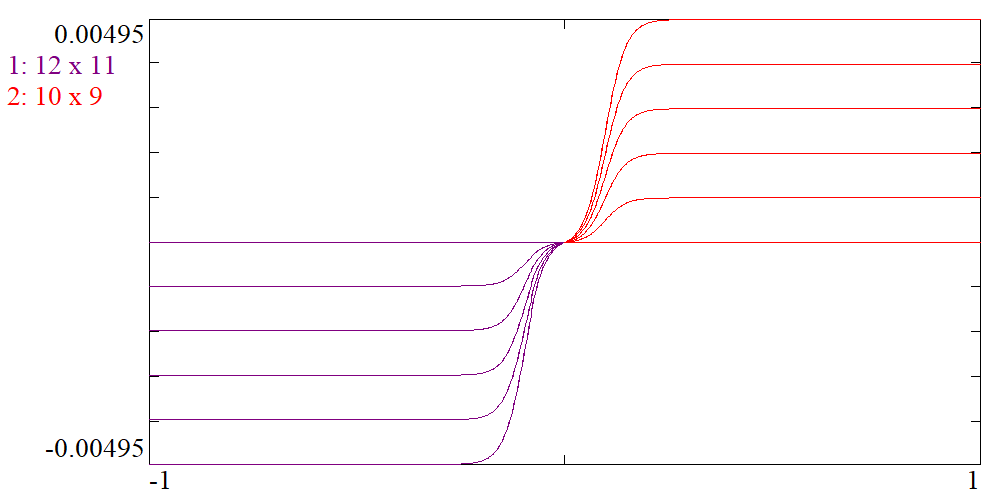
\includegraphics[scale=0.5]{graficos/tracador.png}
\caption{Curvas características do transistor NPN (em vermelho) e PNP (em roxo).}
\end{figure}

\subsubsection{Oscilador Astável com Transistores NPN}

Este circuito, ao ser inicialmente excitado, oscila entre dois pontos de estabilidade, onde um transistor conduz e o outro fica em corte, análogo a uma \textquotedbl gangorra\textquotedbl{}. Assim, por simetria, as curvas das tensões nos coletores ficam iguais, porém deslocadas, demostrando a alternância entre estados.

% Codigo do retificador
\begin{Verbatim}[frame=single]
Oscilador astavel
R1 1 2 1000
R2 1 3 100000
R3 1 4 100000
R4 1 5 1000
C1 3 2 1E-7
C2 5 4 1E-7
Q1 2 4 0 NPN 9.9E-1 5E-1 1E-9 4.3429445E-2 1E-9 4.3429445E-2 1E9
Q2 5 3 0 NPN 9.9E-1 5E-1 1E-9 4.3429445E-2 1E-9 4.3429445E-2 1E9
I1 4 0 PULSE 0 1E-3 1E-3 0 0 1E-3 1000 1
VCC 1 0 DC 10
.TRAN 100E-3 100E-7 TETA 0.55 1
\end{Verbatim}

% Circuito astavel
\begin{figure}[!ht]
\centering
\begin{circuitikz}[scale=0.8] \draw
    (0, 0) node[ground]{}
    (9.5, 0) node[ground]{}
    (0, 2.5) node[npn, xscale=-1, scale=1.5](Q1){}
    (9.5, 2.5) node[npn, scale=1.5](Q2){}
    (Q1.emitter) -- (0,0)
    (Q1.collector) --
    (0, 5) to[R, l=$1 \mathrm{k\Omega}$] (0,8)
    (0, 5) to[C, l_=$100 \mathrm{nF}$, *-]
    (3.5, 5) to[R, l=$100 \mathrm{k\Omega}$]
    (3.5, 8) -- (0,8)
    (Q1.base) --
    (3.5, 2.5) --
    (6, 5) to[C, l_=$100 \mathrm{nF}$, -*]
    (9.5, 5) -- (Q2.collector)
    (3.5, 5) --
    (6, 2.5) -- (Q2.base)
    (Q2.emitter) -- (9.5,0)
    (6, 5) to[R, l_=$100 \mathrm{k\Omega}$]
    (6, 8) -- (12,8)
    (9.5, 8) to[R, l=$1 \mathrm{k\Omega}$]
    (9.5, 5) -- (Q2.collector)
    (3.5, 8) -- (6, 8)
    (12, 8) to[V, l=$10 \mathrm{V}$]
    (12, 5) node[ground]{}
    (-0.5, 5) circle (7pt) node[]{\small{2}}
    (10, 5) circle (7pt) node[]{\small{5}}
    ;
\end{circuitikz}
\caption{Oscilador astável com transistores NPN.}
\end{figure}

\begin{figure}[!ht]
\centering
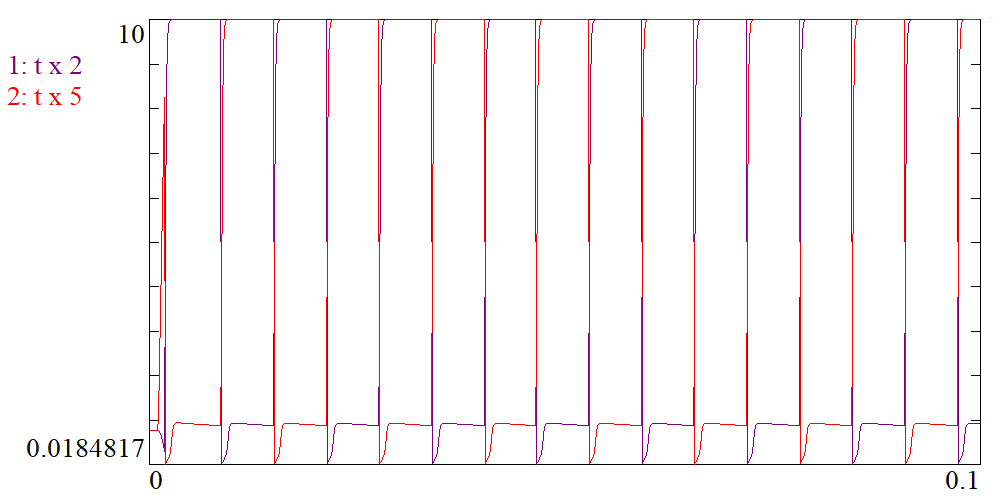
\includegraphics[scale=0.5]{graficos/astavelnpn.png}
\caption{Tensões nos coletores dos dois transistores do oscilador astável. Observe a similaridade entre as curvas.}
\end{figure}



\subsection{Comentários Adicionais}

Antes da conclusão do relatório, é relevante levantar considerações adicionais acerca do desenvolvimento do trabalho, como dificuldades que apareceram no caminho e funcionalidades extra implementadas.

Para evitar o acúmulo de erro numérico associado à adição de valores de ponto flutuante, optou-se por calcular cada tempo de análise como sendo o múltiplo do passo pela posição do ponto na tabela. Essa escolha mostrou também facilitar a construção e depuração do código.

Alguns circuitos trabalham com valores bem baixos para as tensões e correntes, e o algoritmo de Gauss-Jordan com condensação pivotal pode erroneamente encontrar um sistema singular. Para resolver esse problema, foi incluído um bloco de código que diminui a tolerância do método até um valor mínimo, e caso até lá o sistema não convirja é concluído que ele realmente é singular.

É possível que não haja convergência no método de Newton-Raphson caso o chute inicial de valores faça com que os diodos comecem cortados. Isso foi facilmente evitado incluindo uma condição inicial, ou seja, colocando a queda de tensão nos diodos dentro da faixa de condução no início da análise.

Por fim, é importante comentar que foi também implementada uma interface gráfica para o programa usando a API do Windows em C++ (a biblioteca \texttt{windows.h}). Nessa interface é possível refazer a análise de um mesmo arquivo e analisar múltiplos netlists sem precisar reabrir o programa.

\newpage
\section{Conclusão}

O projeto, após ser testado com circuitos \textquotedbl críticos\textquotedbl{} e obter as respostas esperadas, mostrou atingir os objetivos desejados e cumprir as especificações exigidas.

Pôde-se verificar e explorar no trabalho conceitos aprendidos durante a disciplina, como a simplificação de sistemas por amplificadores operacionais, a precisão numérica de aproximações, e a utilidade (e limitações) dos métodos de integração e de Newton-Raphson.

O programa também foi utilizado para a simulação de circuitos de outras disciplinas, obtendo resultados compatíveis com os pretendidos, mostrando-se então uma ferramenta de grande utilidade não só para esta cadeira como também para o restante do curso.

\addcontentsline{toc}{section}{Referências}
\bibliographystyle{ieeetr}
\bibliography{relatorio}


\end{document}